\section*{Results}

\subsection*{Genome assembly and annotation}

We assembled a chromosome-level reference genome for the Pacific acorn barnacle
using PacBio HiFi long reads and Hi-C data.
Preliminary k-mer assessment of the HiFi reads revealed an expected genome
size of $\approx$ 845\,Mbp, with a heterozygosity of over 3\% (Figure~\ref{fig:sup_kmers}).
After purging haplotigs, scaffolding, and polishing the sequences (see
\nameref{sec:methods_assembly}), the final assembly was composed of 592 fragments, and 
had a total sequence length of 1.04\,Gbp and a scaffold N50 of 51.41\,Mbp
(Table~\ref{tab:sup_asm_stats}).
The assembly was 94.08\% gene-complete, with 4.64\% duplicates, for the
\texttt{arthropoda\_odb10} \textsc{BUSCO} dataset
\citep{simao_busco_2015,manni_busco_2021,tegenfeldt_orthodb_2025}.
Of the 1.04\,Gbp assembled, 906.6\,Mbp (86.74\%) was contained in 58 scaffolds
larger than 1\,Mbp.
Moreover, the 16 largest fragments ($>$ 8.5\,Mbp; Figure~\ref{fig:sup_hic})
contained 841.2\,Mbp (80.61\%) of the total sequence, and likely represent 16 chromosomes.
This karyotype number, N=16, is in agreement with that observed for other species in the
genus \textit{Balanus} \citep{austin_chromosome_1958} and other acorn barnacles in the
family Balanidae \citep{han_new_2024}.
\vspace{0.1cm}

Following assembly, we annotated and masked repeat sequences in the genome using
\textsc{EarlGrey} \citep{baril_earl_2024}.
This analysis identified 698.6\,Mbp (66.94\%) of the assembly as repetitive elements
(Table~\ref{tab:sup_earlgrey_summary});
however, the majority of these, 404.5\,Mbp (38.76\% of the assembly), were unable to
be classified among the major repeat families.
This large fraction of unclassified repeats is likely the product of the small number of
representative barnacle sequences among reference repeat databases, further reflecting the
status of barnacles as a genomically understudied group.
Among the classified repeats, DNA and LINE elements were the two most abundant
classes, comprising 8.45\% and 9.16\% of the total assembly, respectively.
\vspace{0.1cm}

We annotated protein-coding genes in the \bgla{} assembly using a combination of
short-read RNAseq and long-read PacBio Iso-Seq data (see
\nameref{sec:methods_protein_coding}).
This process resulted in 20{,}234 protein-coding genes annotated, which had a
\textsc{BUSCO} completeness of 93.58\% and 84.77\% for the \texttt{arthropoda\_odb10}
and \texttt{crustacea\_odb12} datasets, respectively (Table~\ref{tab:sup_annot_stats}).
Comparing this annotation against the proteomes of four other barnacle species (see
\nameref{sec:methods_orthologs}) assigned orthology to 16{,}978 (83.91\%) \bgla{}
protein-coding genes, including 2{,}576 single-copy orthologs across all five species.
In addition to protein-coding genes, we also annotated non-coding elements in the
genome, identifying 7{,}532 long, non-coding RNAs (lncRNA), 1{,}203 transfer RNAs (tRNA),
and 24 ribosomal RNA (rRNA) genes.
In total, across protein-coding and non-coding transcripts, we were able to annotate
28{,}993 genes in the \bgla{} reference assembly.
\vspace{0.1cm}

Together, the high contiguity, gene-completeness, chromosome-level scaffolding,
and comprehensive annotation of this assembly make it among the most complete genomic
resources available for any barnacle species, and a strong foundation for downstream
population genomic and comparative analyses.

\subsection*{Conserved architecture across barnacle genomes}

To assess large-scale structural conservation across barnacle genomes, we performed
a conserved synteny analysis using \textsc{Synolog} \citep{madrigal_synolog_2026}.
We compared our \bgla{} genome against the chromosome-level assemblies of the
striped barnacle \textit{Amphibalanus amphitrite} \citep[Balanidae;][]{han_new_2024}
and the gooseneck barnacle \textit{Pollicipes pollicipes}
\citep[Pollicipedidae;][]{bernot_chromosome-level_2022}.
These genomes display conservation in their large-scale organization, including
one-to-one correspondence between 16 putatively orthologous chromosomes across the
three species (Figure~\ref{fig:synteny}).
Smaller deviations from this one-to-one relationship likely represent assembly errors
are not reflective to changes in chromosomal evolution in these species.
Observing this strong correspondance shows that our scaffolding
of the \bgla{} assembly likely reflects the biological structure of
the genome and is not the product of technical artifacts, and further suggests
conservation of genome architecture across barnacles spanning $\approx$ 165 Mya
of evolution \citep{han_new_2024,bernot_chromosome-level_2022}.
This striking chromosomal stability provides a shared framework for comparative
genomic analyses across the order and suggests that large-scale genome
rearrangements have not been a major driver of diversification in barnacles.

% Synteny
\begin{figure}[ht]
    \centering
    \captionsetup{width=0.95\linewidth}
    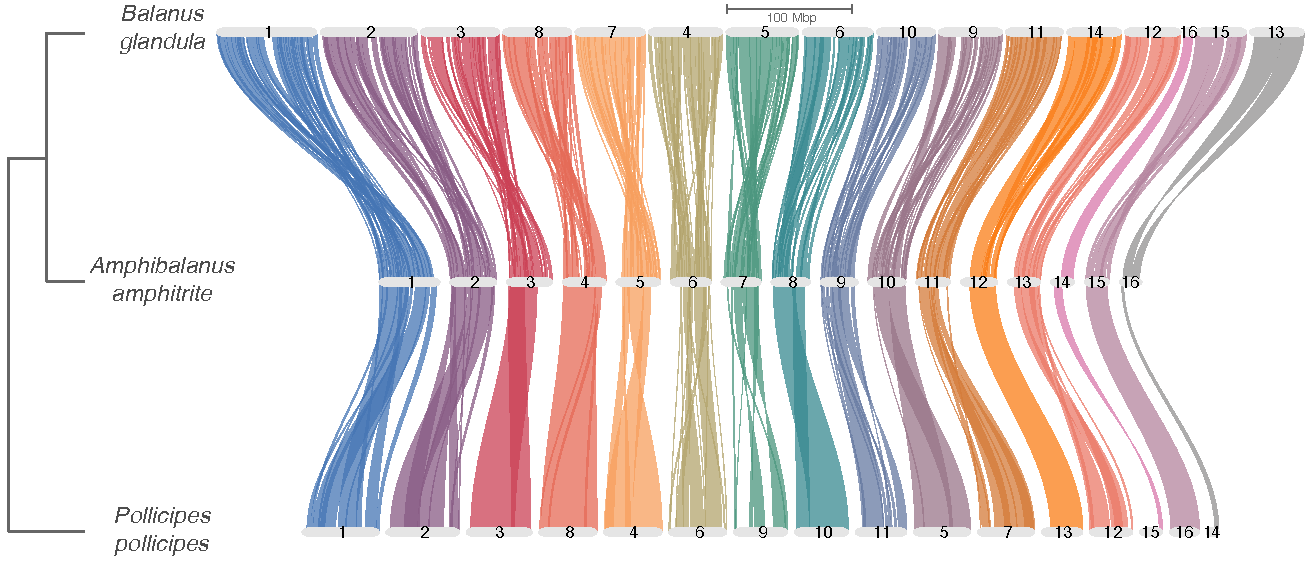
\includegraphics[width=0.95\textwidth]{figures/synteny.pdf}
    \caption{\textbf{Conserved synteny across barnacle genomes.}
        Genome-wide synteny plots showing one-to-one correspondence across
        16 putatively orthologous chromosomes between the genomes of \balgla{}
        (top), \textit{Amphibalanus amphitrite} (middle), and \textit{Pollicipes
        pollicipes} (bottom).
        Each colored line shows protein-coding orthologs across the three
        assemblies, colored according to their chromosome of origin in \bgla{}.
        Cladogram on the left shows the evolutionary relationship among the three
        species.}
    \label{fig:synteny}
\end{figure}

\subsection*{High genetic diversity in the \balgla{} reference assembly}

We estimated the genetic diversity present in the \bgla{} genome by identifying
heterozygous variants in our reference individual. After filtering low-quality sites
and masking regions with annotated repeats, we obtained genotypes for 314 million
sites along the genome, equivalent to 34.71\% of the 904.94\,Mbp present in the 58
scaffolds larger than 1\,Mbp (Table~\ref{tab:sup_popgen_stats}). Among these sites, 
9.08 million (2.89\%) were heterozygous in the reference individual, including 8.73
million SNPs and 356 thousand indels.
In total, this variation represents a mean density of 14.66 heterozygous sites per kbp
(median: 6 per kbp; standard deviation: 19.86).
Moreover, we observed nearly 400 thousand variant sites within protein-coding sequences,
including 144 thousand non-synonymous point mutations.
Transcripts in the reference individual had a mean of 7.74 (median: 3, standard
deviation: 14.97) non-synonymous heterozygous variants, indicating considerable coding
variation segregating within a single individual.
Even from this single genome, the sheer volume of heterozygosity underscores
the exceptionally large population sizes of this species and foreshadows
the extreme diversity observed at the population level.

\subsection*{Functional elements are conserved in barnacle genomes}

We used the \textsc{phastCons} package \citep{siepel_evolutionarily_2005} on the
\textsc{cactus} whole-genome alignment \citep{armstrong_progressive_2020} between
six barnacle species to identify highly conserved elements (HCE) in the Pacific
acorn barnacle genome.
Across the 16 putative chromosomes in the \textit{B. glandula} assembly, \textsc{phastCons}
identified 196{,}141 HCEs, spanning 50.85\,Mbp (6.05\%) of the 16 assembled chromosomes.
In \textit{B. glandula}, the HCEs had a mean length of 259.25\,bp (median: 42\,bp,
standard deviation: 990.40\,bp).
\vspace{0.1cm}

Following the identification of HCEs, we compared their sequence composition against
the genome-wide background (Figure~\ref{fig:phastcons}).
We first intersected the genomic coordinates of the HCEs with the \bgla{}
annotation, obtaining the proportion of annotated features among HCE sites
(Figure~\ref{fig:phastcons}A). Among our target features — which include an
``intergenic'' class for the unannotated fraction of the genome and a ``multiple''
class for overlapping features (e.g., a site spanning both a transposable element
and an intron) — all but one are present among HCEs. We did not observe any conserved
rRNA sites; however, this is likely the product of the whole-genome alignment, given
rRNA's repetitive nature and alignment difficulty \citep{gillespie_characterizing_2004},
and not an accurate measure of conservation (or lack thereof).
Aside from the absence of rRNAs, the sequence composition of HCEs largely followed that
of the whole genome.
Most annotated features do not appear substantially enriched among HCE sites
(Figure~\ref{fig:phastcons}B; Table~\ref{tab:sup_phastcons_enrichment}).
The two clear exceptions are coding sequences (CDSs) and tRNAs.
Protein-coding sequences display an approximately 2-fold enrichment among HCEs (mean
$\log_2$ enrichment: 0.75, median: 0.98, standard deviation: 0.93), reflecting the
conservation of protein-coding genes among barnacle genomes.
Similarly, tRNAs exhibit $\approx$4-fold enrichment in HCEs (mean $\log_2$ enrichment:
2.14, median: 2.04, standard deviation: 0.96), likely reflecting the strong functional
constraints on these sequences.
\vspace{0.1cm}

% Phastcons and enrichment
\begin{figure}[htbp]
    \centering
    \captionsetup{width=0.95\linewidth}
    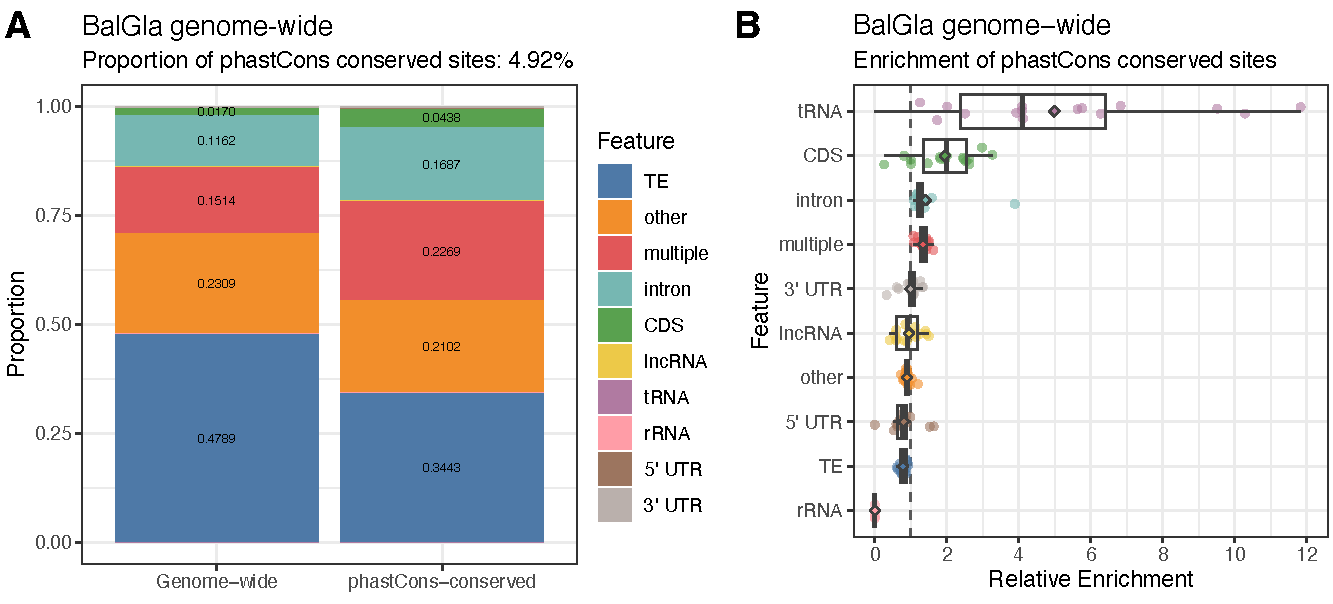
\includegraphics[width=0.9\textwidth]{figures/phastcons.pdf}
    \caption{\textbf{Highly conserved elements in the \balgla{} assembly.}
        \textbf{A.} Proportion of annotated features in the whole genome
        (left column) and the 50.85 Mbp spanning \textsc{phastCons}-conserved elements
        (right column). Values are shown only for elements with proportions larger than
        0.01. Sites that overlap more than one non-intergenic annotation type are
        represented by the ``multiple'' feature.
        \textbf{B.} Enrichment of the annotated features in the highly conserved
        elements compared to the genome-wide background, calculated as the $\log_2$ of
        the relative enrichment. The $\log_2$ enrichment values for each of the 16
        chromosomes are shown as points. The diamonds in the boxplot indicate the
        mean enrichment across the genome.}
    \label{fig:phastcons}
\end{figure}

The enrichment among conserved elements in \bgla{} mirrors patterns observed across other
groups of organisms.
First, coding sequences are consistently enriched among conserved elements, following the
patterns characterized by \citet{siepel_evolutionarily_2005} across vertebrate, insect, worm,
and yeast genomes.
While the raw composition of enriched conserved elements is different across all these
species, the consistent enrichment of CDSs is in accordance with the expectation that
protein-coding sequences are among the most functionally constrained genomic regions.
Secondly, the enrichment pattern in barnacles follows the same ordering observed across
both plants \citep{hupalo_conservation_2013} and animals \citep{siepel_evolutionarily_2005}:
tRNAs are the most enriched annotation among conserved regions, followed by CDSs, while
transposable elements are drastically underrepresented among HCEs.
In contrast, introns are mildly enriched among barnacle HCEs (Figure~\ref{fig:phastcons}B;
Table~\ref{tab:sup_phastcons_enrichment}), while depleted in plant
\citep{hupalo_conservation_2013}, insect, and vertebrate conserved elements
\citep{siepel_evolutionarily_2005}.
However, it remains unknown if this enrichment reflects the larger intronic fraction
of the barnacle genome or genuine intronic conservation in this lineage.
Overall, the conservation of functional elements across barnacle genomes indicates
that purifying selection has been effective at maintaining functionally constrained sequences
despite the highly repetitive nature of the genome, a pattern we revisit in the context
of the broader selective regime acting on these large populations.
% \vspace{0.1cm}

\subsection*{Patterns of molecular evolution reflect positive selection in protein-coding genes}

To examine the rate of molecular evolution in protein-coding sequences, we calculated
the pairwise ratio of non-synonymous to synonymous substitutions (\dnds) between
\bgla{} and its congener, the wrinkled barnacle \textit{Balanus crenatus},
using the codon counting approach described by~\citet{nei1986_dnds}.
We identified and aligned 9{,}082 single-copy orthologs between the two species.
The mean pairwise \dnds{} was 0.206 (median: 0.158, standard deviation: 0.191;
Figure~\ref{fig:sup_dnds}). This ratio indicates that, on average, coding
sequences in these barnacle genomes are under purifying selection, reflecting the
expected evolutionary constraints on sequences of functional importance.
\vspace{0.1cm}

Of the nine thousand genes assessed, 70 (0.77\%) displayed a \dnds{} $>$ 1, and are
likely candidates for positive selection.
The predicted function of the majority ($>80\%$) of these genes is unknown; however,
this is expected, since homology is likely harder to determine for fast-evolving
sequences putatively under strong selection.
Despite this limitation, we found several genes with known function among our positive
selection candidates, including a follistatin-A-like homolog, which is involved
in myogenesis and muscle development in crustaceans \citep{yan_identification_2021}.
We also observed a homolog of $\gamma$-interferon-inducible lysosomal thiol reductase,
which plays a role in crustacean innate immune response \citep{liu_involvement_2019}.
Additionally, we found evidence of positive selection in homologs of tumor protein
p53-inducible protein 11, which is involved in cell cycle regulation and is up-regulated
in crabs after viral infection \citep{cheng_p53_2021}, as well as a Quiver homolog, a
gene related to neuronal activity and sleep regulation in \textit{Drosophila}
\citep{wang_quiver_2010}.
\vspace{0.1cm}

We expanded on our \dnds{} measures of positive selection in protein-coding sequences
in the \bgla{} genome by incorporating population-level polymorphism using the
McDonald-Kreitman (MK) test \citep{mcdonald_adaptive_1991}.
Specifically, we used polymorphism data derived from a population panel of six \bgla{}
individuals from the central Oregon coast (see \nameref{sec:results_popgen}), comparing
those against the orthologous coding sequences in the \textit{B. crenatus} outgroup.
After removing alignments shorter than 100\,bp and those containing premature stop
codons and/or frameshift mutations, we calculated the MK test for 7{,}374 orthologous
sequences between \bgla{} and \textit{B. crenatus}.
\vspace{0.1cm}

Four hundred and forty-four (444, 6.02\%) of these orthologs showed a significant
deviation from the expected proportion of non-synonymous and synonymous substitutions
and polymorphisms (Figure~\ref{fig:mkTest}A).
We additionally calculated the Neutrality Index (NI;~\citealp{rand_excess_1996}) and
Direction of Selection (DoS;~\citealp{stoletzki_estimation_2011}) at each ortholog.
We observed a mean NI value of 0.745 (median: 0.554; standard deviation: 1.079) and
a mean DoS of 0.102 (median: 0.106; standard deviation: 0.131; Figure~\ref{fig:sup_dos}).
Both of these statistics (NI $<1$ and DoS $>0$) show that on average, and in contrast
with our measurements of \dnds{} (see \nameref{sec:discussion_dnds_mkt}), protein-coding
sequences in \bgla{} exhibit an excess of non-synonymous substitutions, suggesting that
they are evolving under positive directional selection when compared to the outgroup sequence.
Moreover, the near absence of genes displaying a significant excess in non-synonymous
polymorphism (NI $>1$) reflect a reduction the proportion of slightly deleterious
variants segregating in the population, suggesting the presence of highly efficacious
background selection.
\vspace{0.1cm}

In addition to NI and DoS, we calculated $\alpha$, a measure of the proportion
of non-synonymous substitutions fixed by positive selection \citep{smith_adaptive_2002}.
We calculated two adjusted versions of $\alpha$ to account for the presence of known
biases.
First, we calculated the Tarone-Greenland $\alpha$ estimator ($\alpha_\text{TG}$), a
weighted estimator that corrects for the effects of averaging over a large number of
genes \citep{stoletzki_estimation_2011}.
Across our 7{,}374 genes, we calculated an $\alpha_\text{TG}$ of 0.540 ($95\%$ CI:
0.534--0.550), which indicates that $\approx$ 54\% of non-synonymous substitutions in
this \bgla{} population were fixed as a product of positive selection.
Secondly, we calculated $\alpha$ using the asymptotic MK test ($\alpha_\text{asym}$),
which corrects for the presence of weakly deleterious non-synonymous polymorphisms
present at low frequency in the population \citep{messer_frequent_2013} which might
obscure the signal of positive selection.
We found a mean $\alpha_\text{asym}$ of 0.610 ($95\%$ CI: 0.610--0.622), a
larger proportion than that observed in \textit{Drosophila} ($\alpha_\text{asym} = 0.57$)
and humans ($\alpha_\text{asym} = 0.13$; \citealp{haller_asymptoticmk_2017,messer_frequent_2013}).
Regardless of the metric used, both $\alpha_\text{TG}$ and $\alpha_\text{asym}$ agree
that the majority of non-synonymous substitutions in this barnacle population are the
outcome of directional positive selection.
Notably, this pervasive signal of positive selection stands in apparent tension with
the low genome-wide \dnds{}, a discordance we address in the \nameref{sec:discussion}.
\vspace{0.1cm}

We explored the predicted function of the candidate genes under positive selection
identified in the MK test by performing a gene ontology (GO) enrichment analysis on the
367 candidates with available functional annotation.
The most enriched GO terms describe a coherent set of cellular functions, spanning the
plasma membrane, adherens junctions, myosin and spectrin complexes, and collagen trimers
(Figure~\ref{fig:mkTest}B;~Figure~\ref{fig:sup_go}).
Among the collagen-related terms, we additionally observe the enrichment of processes
related to the molting of arthropod cuticles (e.g., molting cycle, collagen and
cuticulin-based cuticle).
Together, these enrichment patterns suggest strong directional selection in \bgla{}
on genes involved in the building and remodeling of the cell surface, interactions with
the extracellular matrix, cell-cell adhesion, and related functions.
\vspace{0.1cm}

Several of our candidates under strong positive selection are direct components of these
enriched functions.
For example, two of our top candidates are non-muscle myosin heavy chain and myosin-VIIa homologs,
both showing a very large fraction of non-synonymous substitutions fixed by positive selection,
$\alpha$ of 0.961 and 0.940, respectively.
There is additional evidence of positive selection on proteins with known direct interactions,
such as the components of the spectrin heterodimer, spectrin $\beta$ chain ($\alpha = 0.898$) and
spectrin $\alpha$ chain ($\alpha = 0.895$), the integrin heterodimer, integrin $\alpha$
($\alpha$ = 0.793) and integrin $\beta$ ($\alpha = 0.810$), as well as non-muscle myosin heavy
chain ($\alpha = 0.961$; seen above) and its direct activator Rho-associated protein kinase 1
(ROCK1;~$\alpha = 0.939$).
Observing evidence of positive selection on interacting pairs is strongly suggestive of the
coevolution of these sequences, in a compensatory or correlated fashion; however, future research
is required to fully characterize the molecular interactions produced by these non-synonymous
substitutions in \bgla{}.
\vspace{0.1cm}

Outside of this cell remodeling and adhesion core, the remaining candidates of selection
appear largely functionally heterogeneous, spanning protein synthesis, osmoregulation,
and development (e.g., homologs of eukaryotic translation initiation factor 3 subunits
L and B, transmembrane channel-like 7, and patched domain-containing protein 3-like,
all with $\alpha > 0.9$; \citealp{lee_eif3_2015,liu_osmoregulatory_2025,bolatto_spatial_2015}).
Of these candidates, only a single significant gene in the MK test also appears among our
candidates of selection in the \dnds{} analysis --- a putative homolog of formin-like
protein 3, a member of a family of proteins known to play a role in crustacean immunity
\citep{li_formin-like_2025} --- further highlighting the discrepancy between the two
tests of selection.
Finally, our single candidate showing a significant excess of polymorphism relative to
divergence is a homolog of tubulin $\alpha$-1C chain-like, a major constituent of
microtubules and thus directly linked to the cell-remodeling machinery under positive
selection.
The large excess of polymorphism at this gene (NI = 18.54) instead suggests balancing
selection, and this homolog has additionally been observed as differentially expressed
in response to osmotic stress in barnacles \citep{chandramouli_transcriptome_2015}.

% MK test volcano plot
\begin{figure}[htbp]
    \centering
    \captionsetup{width=0.95\linewidth}
    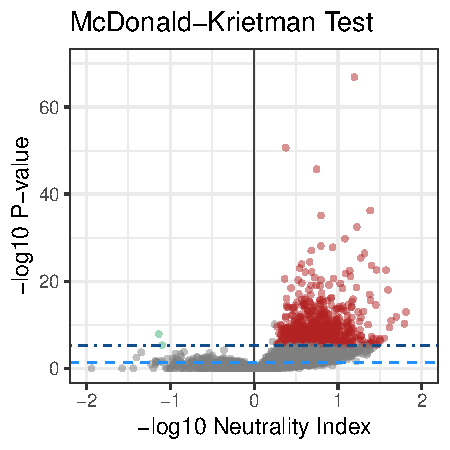
\includegraphics[width=0.95\textwidth]{figures/mkTest.pdf}
    \caption{\textbf{Signatures of positive selection in \balgla{}
        protein-coding genes.}
        \textbf{A.} Selection on 7{,}374 protein-coding genes was assessed using the
        McDonald-Kreitman test.
        X-axis denotes the $-\log_{10}$ of the Neutrality Index, with values on the
        right (NI $<1$) indicating excess of non-synonymous substitutions indicative of
        positive selection.
        Y-axis denotes the $-\log_{10}$ $p$-value of the McDonald-Kreitman test.
        The dashed and dot-dashed lines show the raw ($p<0.05$) and Bonferroni-corrected
        ($p<6.20\times10^{-6}$) significance thresholds, respectively.
        Points in red show the 444 candidates under positive selection, genes with a
        significant excess of fixed non-synonymous substitutions.
        Point in green show the one significant gene with an excess of non-synonymous
        polymorphism.
        \textbf{B.} Significant GO term enrichment among the candidates under
        positive selection in the McDonald-Kreitman test.
        $p_\text{elim}$ denotes the $p$-value calculated from \textsc{topGO}'s
        \texttt{elim} algorithm \citep{alexa_topgo_2006}, which accounts for redundancy
        among GO terms.
        Top, middle, and bottom panels show the top four terms with the largest
        enrichment among the candidates under selection for the three GO categories:
        biological processes, cellular component, and molecular function.}
    \label{fig:mkTest}
\end{figure}

\subsection*{Barnacle genes show biases in the use of synonymous codons}

We compared biases in the usage and composition of synonymous codons in 12 metazoan
genomes, including four barnacles (Table~\ref{tab:sup_enc_summary}), to study the effects of
translational selection in the context of large populations.
Using the annotated transcript sequences in these genomes we calculated the effective number
of codons (ENC), a measure of the extent of departure from equal usage across synonymous
codons \citep{wright_effective_1990,sun_improved_2013}.
In addition to ENC, we also estimated compositional biases by calculating both the overall
coding sequence GC proportion, and the proportion of GC bases at third codon positions (GC3s).
Across 16{,}217 genes in \bgla{}, we find a mean ENC of 43.17 (median: 42.84, standard
deviation: 5.52; Figure~\ref{fig:codon_enc}A;~Table~\ref{tab:sup_enc_summary}).
This number of effective codons is similar to the one observed across three other barnacle
genomes (mean ENC ranging from 42.04 to 44.33; Table~\ref{tab:sup_enc_summary}), highlighting a
substantial reduction in the number of synonymous codon used in barnacles when compared to other
metazoans (Figure~\ref{fig:codon_enc}A).
A similar trend is observed when compared nucleotide composition in barnacle coding sequences
when compared to other metazoans.
All four barnacle genomes studied showed coding sequence GC content of $\approx64\%$, 10 to 20\%
higher than the other studied genomes (Figure~\ref{fig:codon_enc}B;~Table~\ref{tab:sup_enc_summary}).
The higher coding GC proportion in barnacles is also observed when looking at the GC proportion
at 3rd codon positions and at 4-fold degenerate sites (Figure~\ref{fig:sup_coding_gc}).
\vspace{0.1cm}

We explored the selective basis of the increased bias in codon usage in barnacle genomes by
comparing the empirical ENC distribution against a theoretical expectation.
In its original definition of the ENC statistic, \citet{wright_effective_1990} devised a
relationship between GC3s and ENC, resulting in an expected number of effective codons for a
given GC content.
Deviations from this expectation, specifically observing a smaller number of effective codons
than expected, suggest the presence of strong translational selection acting on the genome.
After testing this relationship across these 12 genomes, we observe that the reduction in
the number of effective codons observed in barnacles can in most cases be explained by their
coding GC proportion (Figure~\ref{fig:sup_enc_gc3s}; Figure~\ref{fig:sup_enc_reg}), suggesting
a codon usage bias driven by neutral processes.
In \bgla{} specifically, we observed a moderate deviation when comparing the empirical ENC
distribution against Wright's curve (Figure~\ref{fig:codon_enc}C); however, when comparing the
linear relationship between observed and expected ENC, a better fit for GC biased genomes such
as \bgla{}, we do observe a reduction in the model's slope and coefficient of determination
($\text{R}^2$; Figure~\ref{fig:codon_enc}D).
This poorer fit of the model indicates a smaller than expected number of effective codons, and
suggests the presence of strong translational selection acting on the genome and the potential
non-neutrality of at least some synonymous codons in large \bgla{} populations.
\vspace{0.1cm}

Comparing the ENC and GC3s distribution in relation to population size highlights some
interesting patterns.
Evidence for selection-driven codon usage biases is observed for some hyper-diverse, large
population species, e.g., the nematode \textit{Caenorhabditis brenneri}, the Pacific oyster
\textit{Magallana gigas}, and the European lancelet \textit{Branchiostoma lanceolatum}
(Figure~\ref{fig:sup_enc_gc3s}; Figure~\ref{fig:sup_enc_reg}; Table~\ref{tab:sup_enc_models}).
More moderate deviation is observed for other diverse species, e.g, the malaria mosquito
\textit{Anopheles gambiae} and the tunicate \textit{Ciona intestinalis}.
In contrast, in three of our studied barnacles (\textit{B. crenatus}, \textit{A. amphitrite},
and \textit{P. pollicipes}), the observed codon usage biases appear are indistinguishable from
neutral compositional processes.
In \bgla{}, evidence for non-neutral codon usage biases is moderate to strong depending on the
method used.
Overall, while we do not observe a clear relationship between population size and codon usage
biases in the 12 studied genomes, the lineage-specific patterns described here provide an
unexplored avenue of study of the efficacy and breadth of selection in highly diverse genomes.

% ENC codon bias
\begin{figure}[htbp]
    \centering
    \captionsetup{width=0.95\linewidth}
    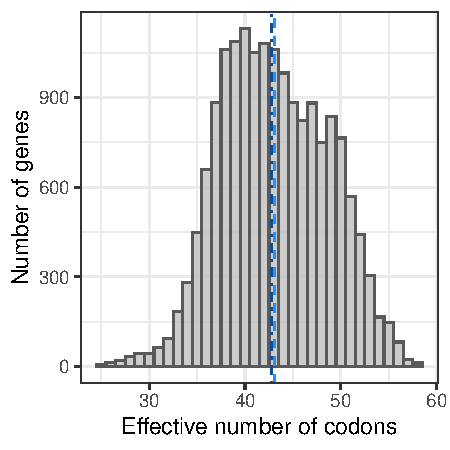
\includegraphics[width=0.9\textwidth]{figures/codon_bias.pdf}
    \caption{\textbf{Codon usage biases in \balgla.}
        \textbf{A.} Genome-wide distribution of the effective number of codons (ENC)
        in \bgla{} (\texttt{BalGla}) and other metazoan genomes (see Table~\ref{tab:sup_enc_summary}),
        including the barnacles \textit{B. crenatus} (\texttt{BalCre}), \textit{A. amphitrite}
        (\texttt{AmpAmp}), and \textit{P. pollicipes} (\texttt{PolPol}).
        The vertical lines show the 50\textsuperscript{th} quantile (median) of the
        distribution, while the crosses show the mean value.
        \textbf{B.} Distribution in the proportion of GC bases in coding sequences
        of 12 metazoan genomes. Vertical lines and crosses show the mean and median
        values, respectively.
        \textbf{C.} Relationship between the GC proportion at the 3rd codon site (GC3s)
        and ENC in \bgla{}. Each black dot represents a gene, while the red curve shows
        the expected relationship in accordance with Wright's curve
        \citep{wright_effective_1990}. Points below the curve show genes with a smaller
        than expected number of effective codons, candidates for translational selection.
        \textbf{D.} Relationship between the expected number of effective codons (according
        to Wright's curve) and the empirical ENC distribution in \bgla{}. Red line shows the
        linear regression between expected and observed ENC distributions.}
    \label{fig:codon_enc}
\end{figure}

\subsection*{Barnacle populations exhibit elevated genetic polymorphism}\label{sec:results_popgen}

We sequenced the whole genomes of eight \bgla{} individuals from the central Oregon coast
using Illumina short reads.
After removal of two samples with poor quality sequences, and the stringent filtering of
sites with low coverage, low quality, and/or missing genotypes, we recovered a total of
111.6 million genotyped sites (Table~\ref{tab:sup_popgen_stats}), 21.4 million (19.16\%)
of which were variant in the six retained samples.
Among these variant sites, we recovered 20.5 million point mutations, 4.86\% of which 
were multiallelic in just these six individuals.
In total, the amount of polymorphism observed in our sampling translates to a mean
density of 41.1 variant sites per kbp (median: 29, standard deviation: 40.82).
Moreover, 1.1 million of these variant sites (5.23\%) were located in coding sequences.
These coding variants included 360 thousand missense (non-synonymous) mutations,
corresponding to a mean of 18.93 non-synonymous variants per transcript
(median: 10, standard deviation: 28.50).
Overall, these represent a substantial proportion of coding variation segregating in
central Oregon.
This \bgla{} population displayed a mean genome-wide nucleotide
diversity ($\pi$) of 0.0506 (median: 0.0531, standard deviation: 0.0188;
Figure~\ref{fig:genome_pi}; Table~\ref{tab:sup_feature_pi}).
For context, this magnitude of $\pi$ is approximately $4\times$ higher than that
observed in \textit{Anopheles gambiae} mosquitos, a species known for their high
levels of polymorphism, $\approx7\times$ higher than the diversity in Sub-Saharan
populations of \textit{Drosophila melanogaster}, and $\approx48\times$ higher than the
diversity observed in large human cohorts~(Figure~\ref{fig:sup_pi_comp}).
\vspace{0.1cm}

Along each chromosome, we did not observe any strong correlation between the density
of specific genomic features (e.g., CDSs, lncRNAs, tRNAs, introns, and repeats) and
$\pi$, particularly not at the scale of 10\,kbp (Figure~\ref{fig:genome_pi};
Figure~\ref{fig:sup_pi_pairplot}).
However, stronger relationships are likely present at other genomic intervals given
the differences in diversity seen across genetic elements (see below).
The strongest correlation was, expectedly, observed between the density of segregating sites
within 10\,kbp windows and $\pi$ (Spearman's $\rho$: 0.706; Figure~\ref{fig:sup_pi_pairplot}).
The proportion of segregating sites in itself was not correlated with the density of
particular genomic features, except for repeats; however, this is likely an artifact of the
masking of genotypes located within repetitive intervals in the reference
(see \nameref{sec:methods_popgen}).
Despite the lack of clear correlation, the patterns of $\pi$ observed along
the chromosomes are qualitatively similar to those expected under regimes of
strong linked selection, in which regions of reduced diversity are the result
of differences in the recombination landscape (e.g., reduction in recombination
in centromeric regions).
Describing recombination in detail this species should thus be a focus of future studies
in order to characterize how highly efficacious selection and linkage shape genetic
diversity along the genome in \bgla{}.
\vspace{0.1cm}

% Genome-wide pi & repeat and gene density
\begin{figure}[htbp]
    \centering
    \captionsetup{width=0.95\linewidth}
    \includegraphics[width=1.0\textwidth]{figures/genome_pi.pdf}
    \caption{\textbf{Nucleotide diversity ($\pi$) and coding and repeat density
        along the \balgla{} genome.}
        \textbf{A.} Density of coding sequences (CDS) along the genome, defined as the
        proportion of bases annotated as CDS within 10\,kbp windows. Line reflects the
        kernel-smoothed values along a 1\,Mbp window. Dashed horizontal line shows
        the genome-wide average proportion of CDS bases (0.0288). Top and bottom
        horizontal axes show the chromosome number and genomic position, respectively.
        \textbf{B.} Density of repeat elements annotated within 10\,kbp windows, smoothed
        along 1\,Mbp intervals. Dashed horizontal line shows the genome-wide average
        proportion of repeat bases (0.597).
        \textbf{C.} Density of segregating sites, calculated as the proportion of SNPs
        within 10\,kbp windows, smoothed along 1\,Mbp intervals. Dashed horizontal line
        shows the genome-wide average proportion of segregating SNPs per 10\,kbp
        (0.0307).
        \textbf{D.} $\pi$ within 10\,kbp windows, smoothed along 1\,Mbp intervals.
        Horizontal dashed line shows the mean genome-wide $\pi$ (0.0506).}
    \label{fig:genome_pi}
\end{figure}

Looking at diversity across the genome, we observed an overall reduction in $\pi$
at putatively functional sites. For example, the mean $\pi$ in sequences spanning
annotated CDSs is 0.0302 (median: 0.0270, standard deviation: 0.0221;
Figure~\ref{fig:feature_pi}; Table~\ref{tab:sup_feature_pi}),
which represents a $\approx1.6\times$ reduction in diversity when compared to the
genome-wide average. A reduction in diversity of similar magnitude is also observed
in the sequences of lncRNAs ($1.4\times$) and 5' UTRs ($1.3\times$). The largest reduction
in diversity when compared to the genome-wide background was observed in tRNAs, with
$\pi~\approx4.3\times$ lower than the genomic background and consistent with the
strong functional constraint evidenced by their enrichment in highly conserved elements.
In contrast to most other elements of the genome, introns display a relative increase in
diversity, with a mean $\pi$ of 0.0646 (median: 0.0650, standard deviation: 0.0299),
approximately $1.3\times$ higher than the genome-wide average.
\vspace{0.1cm}

Zooming in further on coding sequences, we explored the patterns of $\pi$
at 0-fold degenerate ($\pi_{0}$), in which any mutation produces a non-synonymous
substitution, and 4-fold degenerate sites ($\pi_{4}$), in which any mutation results
in a synonymous change.
This comparison allows us to compare diversity at constrained versus neutral (or
putatively neutral) sites.
In this central Oregon population of \bgla{}, the mean $\pi_{0}$, was 0.0107 (median:
0.00292, standard deviation: 0.0178).
This is the lowest diversity among the studied categories in the genome, not a
surprising result given the higher functional constraint expected at these sites.
In contrast, mean $\pi_{4}$ was 0.0790 (median: 0.0750, standard deviation: 0.0483),
$\approx1.6\times$ higher than the genome-wide average and the highest in the genome.
The nearly 8-fold difference between $\pi_{0}$ and $\pi_{4}$ highlights the
strong constraint on non-synonymous sites and suggests that purifying selection is
highly effective in this population, consistent with theoretical predictions for
species with large effective population sizes.

% Distribution of pi for different features in the genome
\begin{figure}[htbp]
    \centering
    \captionsetup{width=0.95\linewidth}
    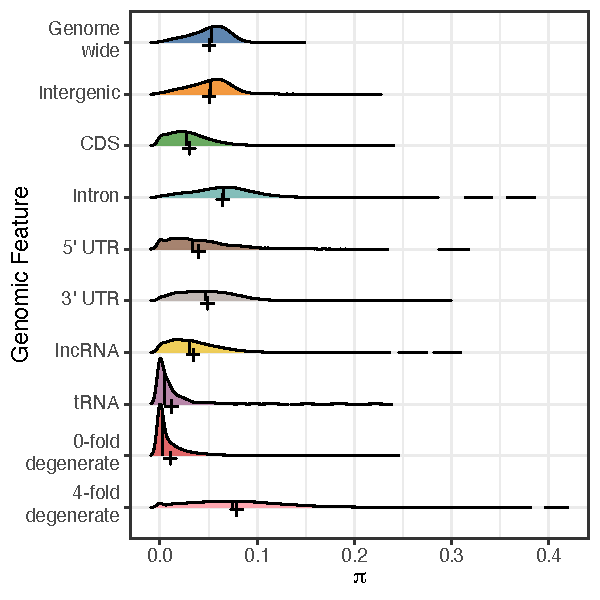
\includegraphics[width=0.6\textwidth]{figures/feature_pi.pdf}
    \caption{\textbf{Nucleotide diversity ($\pi$) across genomic
        features in Oregon \balgla.}
        The density histogram shows the distribution of windowed
        $\pi$ values across different genomic features annotated
        in the \bgla{} assembly. The vertical lines show the
        50\textsuperscript{th} quantile (median) of the distribution,
        while the crosses show the mean value.}
    \label{fig:feature_pi}
\end{figure}

\subsection*{\balgla{} exhibits large effective population sizes}

We estimated the effective population size (\Ne{}) for a central
Oregon \textit{B. glandula} population sample using the whole-genome genotypes.
As a simple estimate of the long-term \Ne{} of this population, we first
calculated \Ne{} using Watterson's estimator of genetic diversity ($\theta_\text{W}$),
observing a mean genome-wide $\theta_\text{W}$ of 0.0617 (median: 0.0635, standard
deviation: 0.0224; Figure~\ref{fig:sup_theta_ne}). Assuming a per-base,
per-generation mutation rate ($\mu$) of $3\times10^{-9}$ (as estimated by
\cite{nunez_footprints_2020} for the northern acorn barnacle \textit{S. balanoides})
and using the relationship between \Ne{} and $\theta_\text{W}$, this yields a
mean effective size of 5{,}137{,}172 (median: 5{,}289{,}211, standard deviation:
1{,}862{,}683), which is consistent with the expectation of large \Ne{} in this species.
\vspace{0.1cm}

Additionally, we estimated \Ne{} through time using a coalescent-based
approach with \textsc{msmc2} \citep{dutheil_msmc_2020}. This estimate also placed
the historical effective size of the population on the order of $10^{6}$ individuals
(between $10^{6}$ and $10^{7}$ generations ago) (Figure~\ref{fig:sup_mcmc_ne});
however, given our small sample size and the use of only within sample pairwise
comparisons, we were unable to obtain accurate \Ne{} estimates at more recent
($<10^{5}$ generations) timescales using \textsc{msmc2}.
Nevertheless, even these conservative estimates place \bgla{} among the
largest known effective population sizes for any eukaryote, yet orders of
magnitude below the census sizes observed in the field --- a disparity
central to Lewontin's Paradox and one we return to in the Discussion.
